\section{Auswertung}
\label{sec:Auswertung}

\subsection{Messwerte:}
Im nachfolgenden sind alle Messwerte tabellarisch dargestellt:
\begin{table}
\centering
\caption{Mischen der Signale:}
\label{tab:data2}
\sisetup{table-format=1.2}
\begin{tabular}{S[table-format=3.0] S S S S[table-format=3.2]}
\toprule
{$\phi [deg]$} & {$U_{out}[V]$} & {$Tiefpass [V] - gainbereinigt$}\\
\midrule
0 & 3.04 & 1.5 \\
45 & 4.60 & 0.9 \\
90 & 4.92 & -0.3 \\
135 & 3.92 & -1.25 \\
180 & 3.04 & -1.5 \\
210 & 4.04 & -1.25 \\
270 & 4.92 & 0.3 \\
340 & 2.52 & 1.5 \\
\bottomrule
\end{tabular}
\end{table}

\begin{table}
\centering
\caption{Rauschgenerator:}
\label{tab:data3}
\sisetup{table-format=1.2}
\begin{tabular}{S[table-format=3.0] S S S S[table-format=3.2]}
\toprule
{$\phi [deg]$} & {$U_{out}[V]$} & {$Tiefpass [V ]- gainbereinigt$}\\
\midrule
0 & 3.20 & 1.5 \\
45 & 4.84 & 0.9 \\
90 & 5.20 & -0.3 \\
135 & 4.21 & -1.25 \\
180 & 3.32 & -1.5 \\
210 & 4.28 & -1.25 \\
270 & 5.16 & 0.3 \\
340 & 2.92 & 1.5 \\
\bottomrule
\end{tabular}
\end{table}

\begin{table}
\centering
\caption{LED und Photodiode:}
\label{tab:data4}
\sisetup{table-format=1.2}
\begin{tabular}{S[table-format=3.0] S S S S[table-format=3.2]}
\toprule
{$r [cm]$} & {$Tiefpass [V]$} & {$Gain (Tiefpass)$}\\
\midrule
6 & 3.6 & 20 \\
16 & 2.1 & 50 \\
26 & 3.1 & 200 \\
36 & 3.9 & 500 \\
46 & 4.5 & 1000 \\
56 & 3.1 & 1000 \\
66 & 2.3 & 1000 \\
76 & 1.9 & 1000 \\
86 & 1.5 & 1000 \\
96 & 1.1 & 1000 \\
106 & 1.0 & 1000 \\
116 & 0,9 & 1000 \\
126 & 0,9 & 1000 \\
146 & 0,6 & 1000 \\
166 & 0,5 & 1000 \\
186 & 0,5 & 1000  \\
\bottomrule
\end{tabular}
\end{table}
\newpage

\newpage

\subsection{Auswertung: Funktionsgenerator}
Die Messung ergibt eine gleichbleibende Spannungsamplitude von 4,48V für den
rechten Ausgang.
Am linken Ausgang lässt sich die Spannungsamplitude von 0V
bis zu der Amplitude des
anderen Ausgangs regeln, also maximal 4,48V.

\subsection{Auswertung: Mischen der Signale}

Die Signalspannung wird im folgenden mit einer Amplitude von 1V und einer
Frequenz von 1kHz betrieben. Als Amplitude wird hierbei die Spannung zwischen
oberer und unterer Halbwelle bezeichnet; als Phasenverschiebung der Wert, der am
Gerät eingestellt wird. Die interne Phasenverschiebung wird zunächst
vernachlässigt. Als Beispiel dient ein Messwert, der bei $\phi = 0°$
aufgezeichnet wurde, die Amplitude der Ausgangsspannung beträgt 3,04V:
\begin{figure}[H]
  \centering
  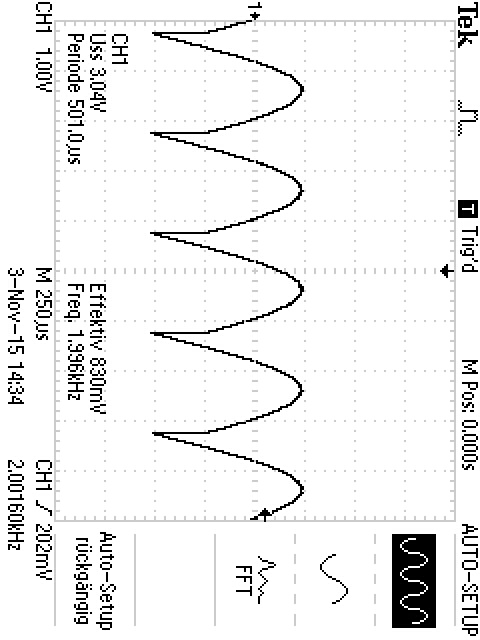
\includegraphics[angle=90,height=0.3\textwidth,width=0.6\textwidth]
  {graphics/ALL0031/F0031TEK.jpg}
  \caption{$U_{out}$ für $\phi$=0}
  \label{fig:2/phi0}
\end{figure}

In Abb.\ref{fig:plot2u} ist die gemischte Ausgangsspannung $U_{out}$ gegen die
Phasenverschiebung $\phi$ aufgetragen. Gut zu erkennen ist die Abhängigkeit
der Ausgangsspannung von der Phasenverschiebung. Die Maxima von $U_{out}$
liegen hierbei bei etwa 90° bzw. 270°:
\begin{figure}[H]
  \centering
  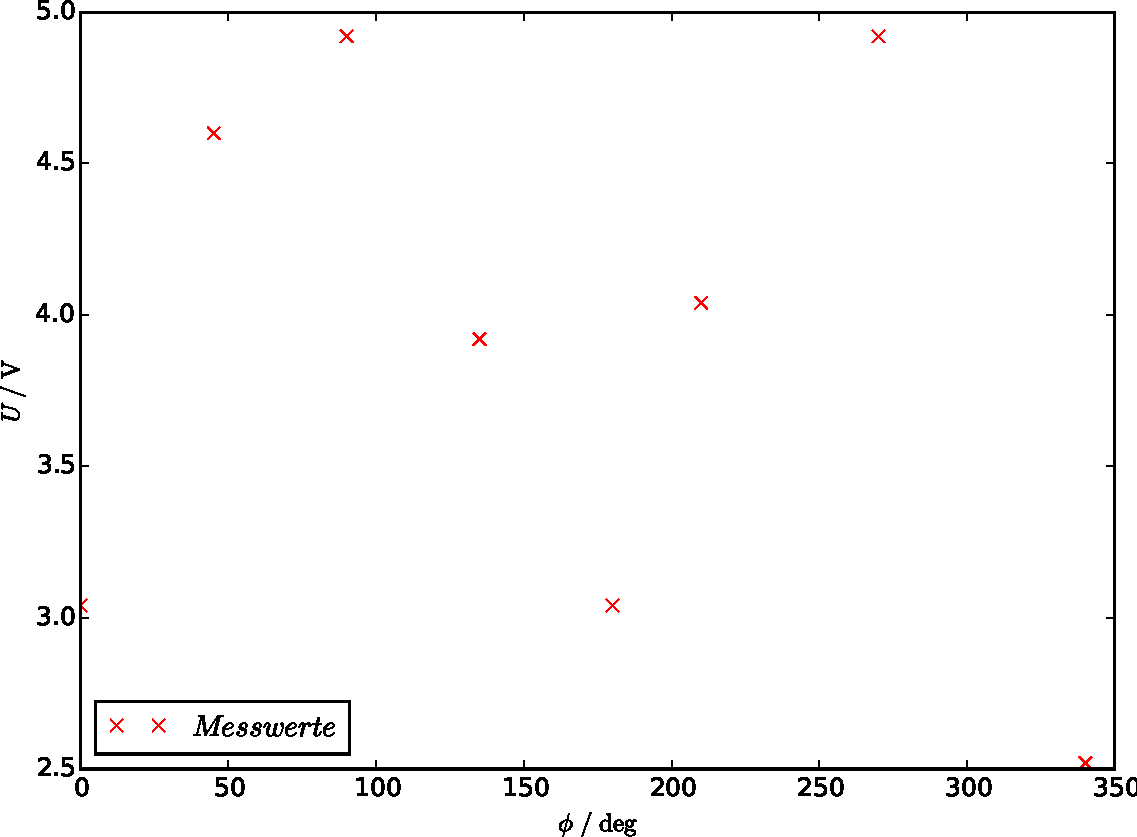
\includegraphics[width=0.65\textwidth, height=0.35\textwidth]{plot2u.pdf}
  \caption{$U_{out}$ nach Mischen ohne Rauschen}
  \label{fig:plot2u}
\end{figure}
\newpage
In Abb.\ref{fig:plot2low} ist das am Tiefpaß integrierte Signal gegen die
Phasenverschiebung $\phi$ aufgetragen. Maximale Werte ergeben sich um $\phi = 0°$
herum, das Minimum liegt bei ca. $\phi = 180°$. Das deckt sich mit der Formel
\eqref{eqn:Uout}, in der $\phi$ in einem Cosinus auftaucht.
\begin{figure}[H]
  \centering
  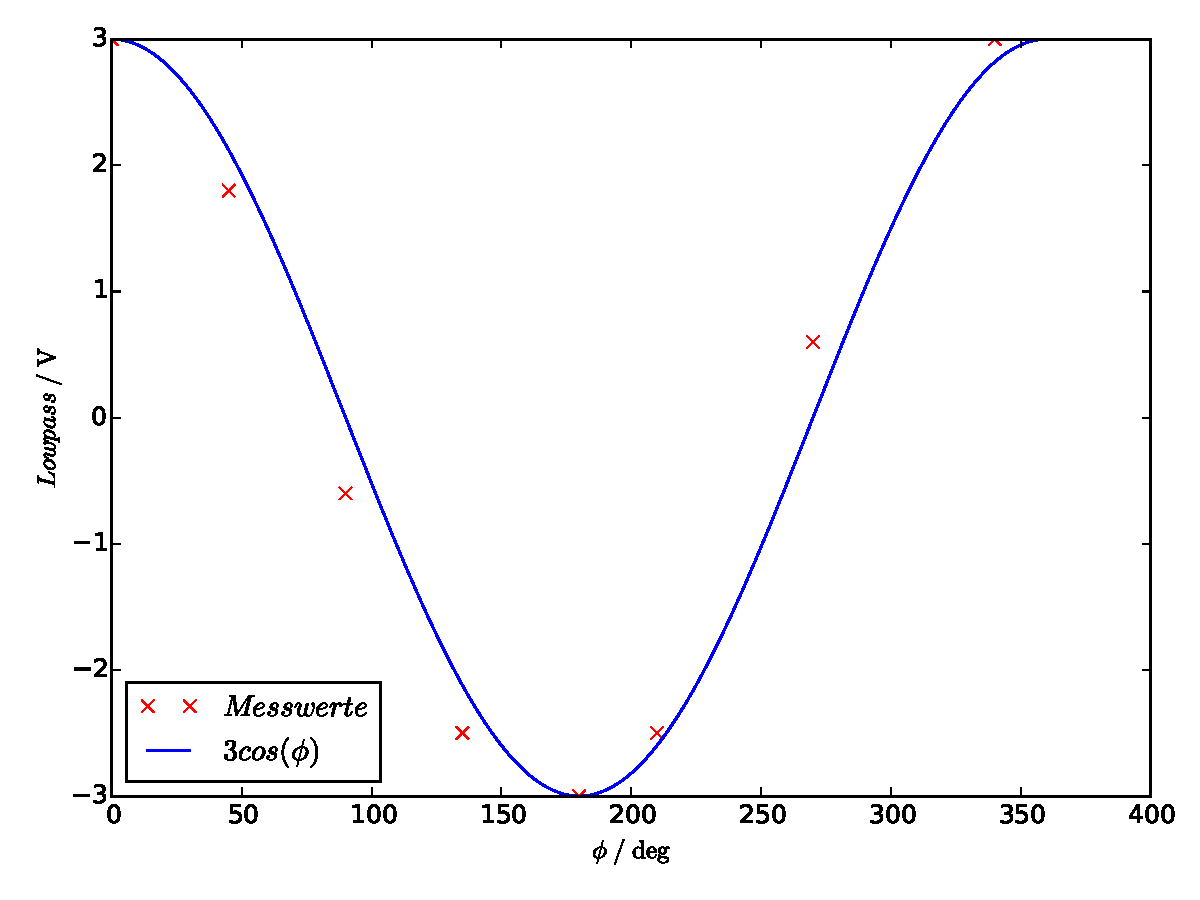
\includegraphics[height=0.35\textwidth,width=0.65\textwidth]{plot2low.pdf}
  \caption{Integral der gemischten Ausgangsspannung ohne Rauschen}
  \label{fig:plot2low}
\end{figure}


\subsection{Auswertung: Rauschgenerator}

Wie unschwer in Abb.\ref{fig:3/phi0} zu erkennnen ist, ergeben sich mit Rauschen
sehr ähnliche
Messwerte nach Filterung und Mischen. Im folgender Abbildung ist die
Spannung für $\phi=0°$ dargestellt, analog zu Abb.\ref{fig:2/phi0}.

\begin{figure}[H]
  \centering
  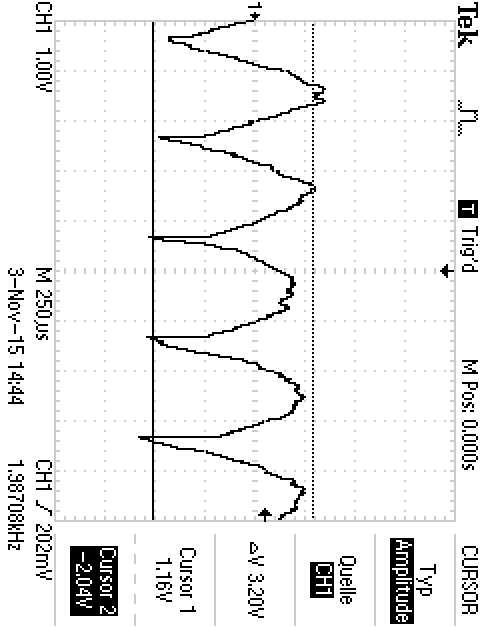
\includegraphics[angle=90,width=0.6\textwidth, height=0.3\textwidth]{graphics/ALL0039/F0039TEK.jpg}
  \caption{$U_{out}$ für $\phi$=0 mit Rauschen}
  \label{fig:3/phi0}
\end{figure}

Gut sichtbar ist das nicht vollständig rausgefilterte Rauschen in Abb.
\ref{fig:3/phi0}, die Form der
Spannungskurve ähnelt aber stark der aus Abb.\ref{fig:2/phi0}.

\newpage
Für $U_{out}$ ergeben sich folgende Messwerte in Abhängigkeit von $\phi$:

\begin{figure}[H]
  \centering
  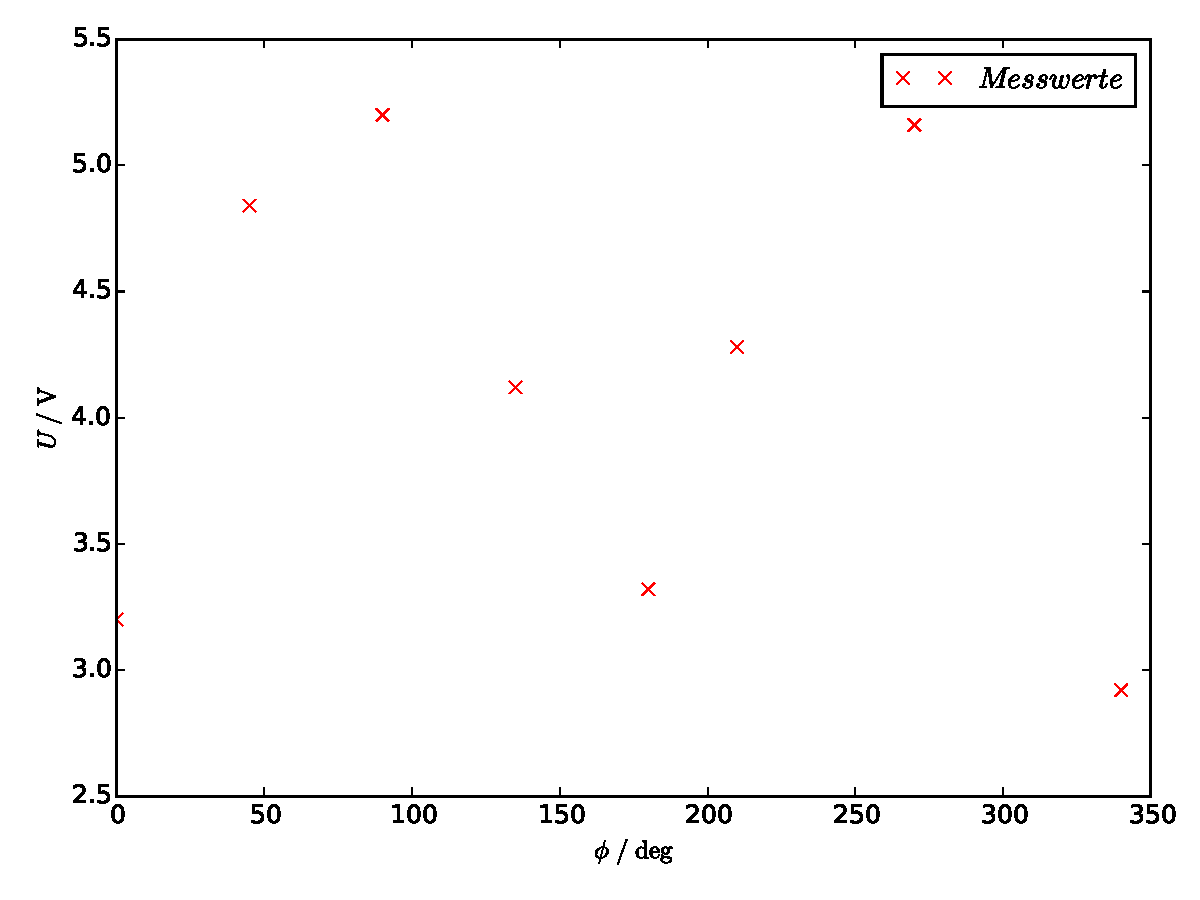
\includegraphics[width=0.65\textwidth, height=0.35\textwidth]{plot3u.pdf}
  \caption{$U_{out}$ nach Mischen mit Rauschen}
  \label{fig:plot3u}
\end{figure}

Die Messwerte an dem Tiefpaß (Abb.\ref{fig:plot3low}) unterscheiden sich
überhaupt nicht von denen ohne zugeschalteten
Rauschgenerator (Abb.\ref{fig:plot2low}).
Der Grund dafür ist, dass der Tiefpaß die Spannung über mehrere
Periodendauern integriert. Daher wird das verbliebene Rauschen einfach
herausgemittelt.
\begin{figure}[H]
  \centering
  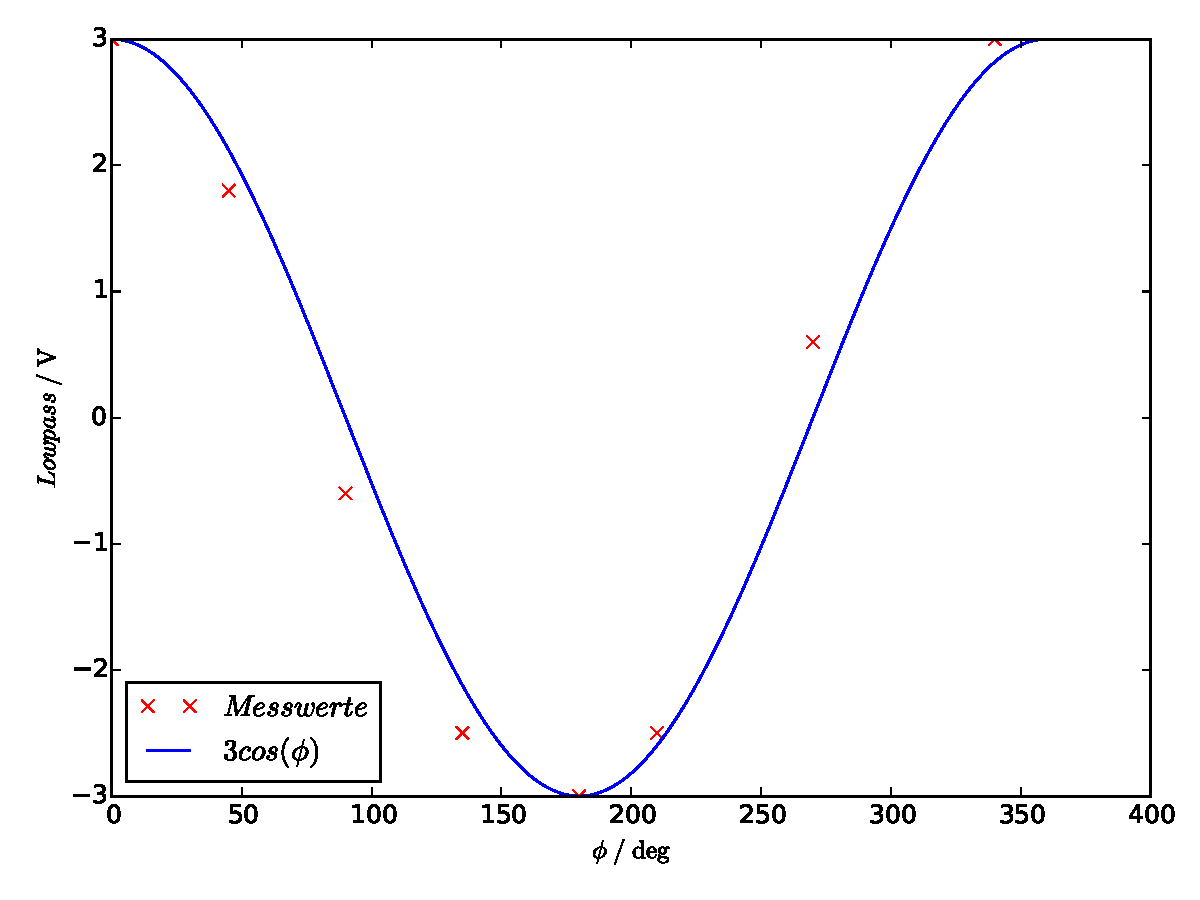
\includegraphics[width=0.65\textwidth, height=0.35\textwidth]{plot3low.pdf}
  \caption{Integral der gemischten Ausgangsspannung mit Rauschen}
  \label{fig:plot3low}
\end{figure}
Auf den folgenden zwei Seiten sind alle Meßwerte für $U_{out}$
(mit und ohne Rauschen; vor der Integration am Tiefpaß) dargestellt:
\newpage
\hspace{-3cm}
\captionsetup{labelformat=empty}
\begin{figure}[H]
  \caption*{$U_{out} ( \phi = 0°$) }
  \centering
  \begin{subfigure}{0.48\textwidth}
      \centering
      \caption*{ohne Rauschen:}
      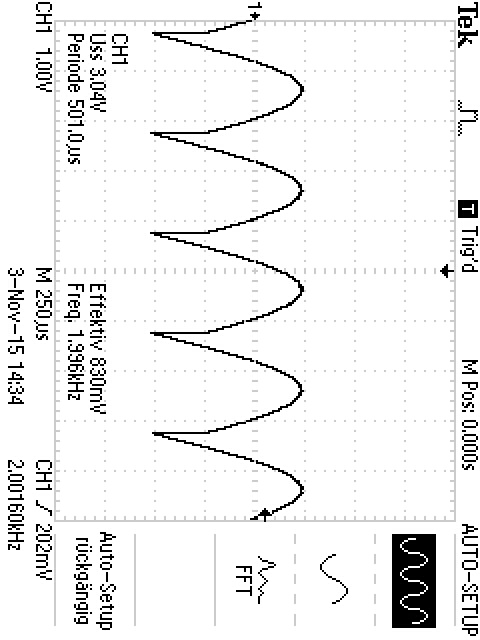
\includegraphics[angle=90,height=2.6cm]{graphics/ALL0031/F0031TEK.jpg}
  \end{subfigure}
  \begin{subfigure}{0.48\textwidth}
      \centering
      \caption*{mit Rauschen:}
      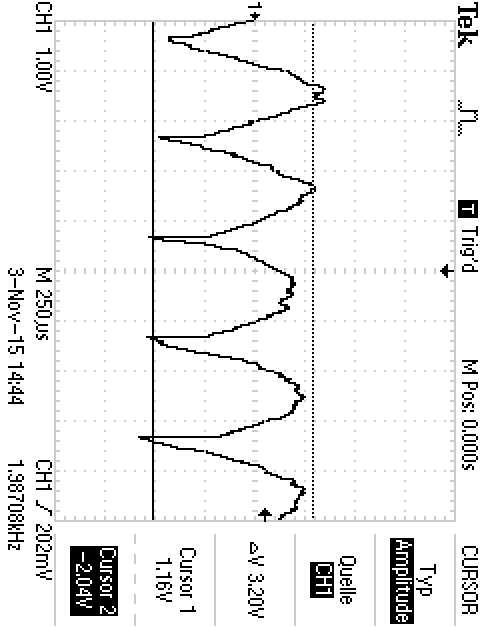
\includegraphics[angle=90,height=2.6cm]{graphics/ALL0039/F0039TEK.jpg}
  \end{subfigure}
\end{figure}
\addtocounter{figure}{-1}
\begin{figure}
\caption{$U_{out} (\phi = 45°$) }
\begin{subfigure}{0.48\textwidth}
\centering
\caption*{ohne Rauschen:}
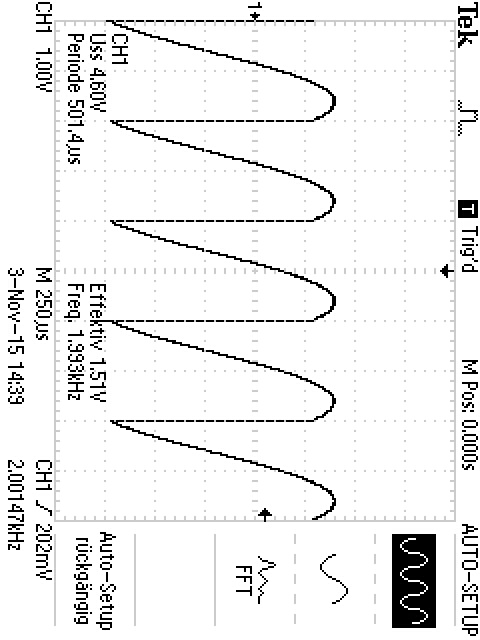
\includegraphics[angle=90,height=2.6cm]{graphics/ALL0037/F0037TEK.jpg}
\label{fig:phi45o}
\end{subfigure}
\begin{subfigure}{0.48\textwidth}
\centering
\caption*{mit Rauschen:}
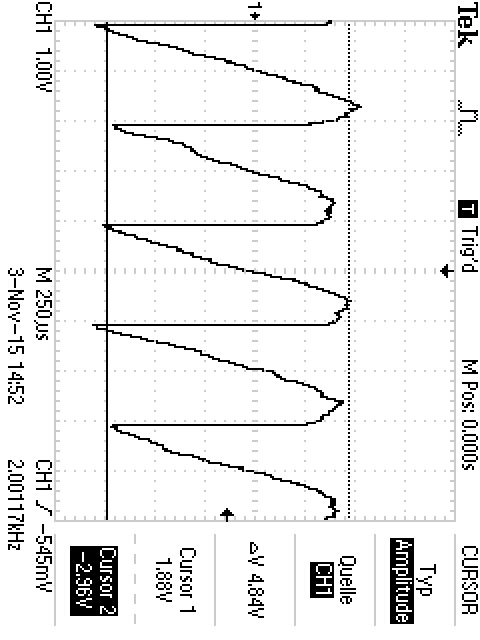
\includegraphics[angle=90,height=2.6cm]{graphics/ALL0045/F0045TEK.jpg}
\label{fig:phi45m}
\end{subfigure}
\end{figure}
\addtocounter{figure}{-1}
\begin{figure}
\caption{$U_{out} (\phi = 90°$) }
\begin{subfigure}{0.48\textwidth}
\centering
\caption*{ohne Rauschen:}
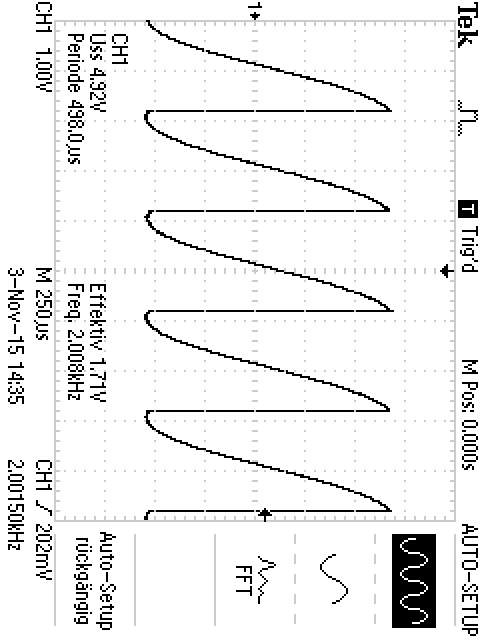
\includegraphics[angle=90,height=2.6cm]{graphics/ALL0033/F0033TEK.jpg}
\label{fig:phi90o}
\end{subfigure}
\begin{subfigure}{0.48\textwidth}
\centering
\caption*{mit Rauschen:}
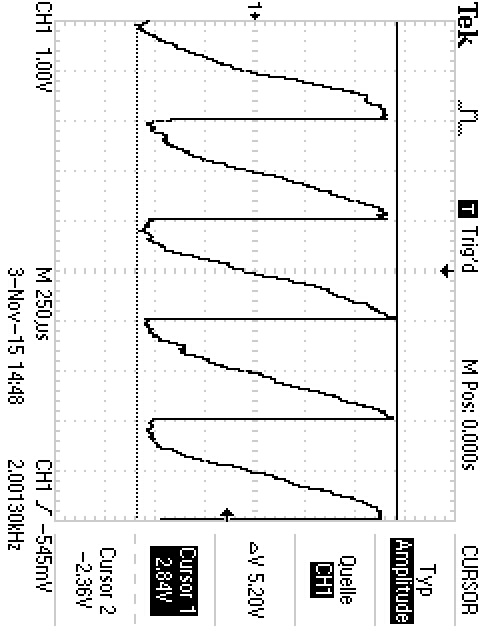
\includegraphics[angle=90,height=2.6cm]{graphics/ALL0041/F0041TEK.jpg}
\label{fig:phi90m}
\end{subfigure}
\end{figure}
\addtocounter{figure}{-1}
\begin{figure}
\caption{$U_{out} (\phi = 135°$)}
\begin{subfigure}{0.48\textwidth}
\centering
\caption*{ohne Rauschen:}
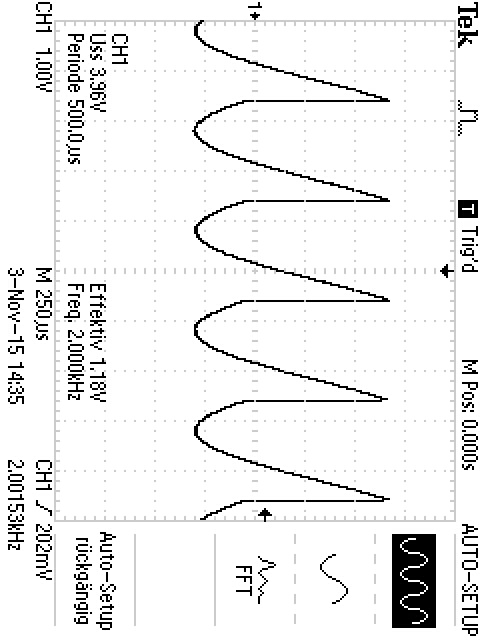
\includegraphics[angle=90,height=2.6cm]{graphics/ALL0032/F0032TEK.jpg}
\label{fig:phi135o}
\end{subfigure}
\begin{subfigure}{0.48\textwidth}
\centering
\caption*{mit Rauschen:}
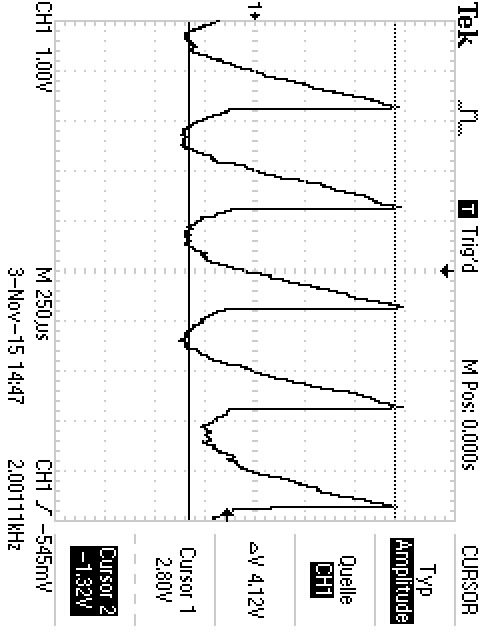
\includegraphics[angle=90,height=2.6cm]{graphics/ALL0040/F0040TEK.jpg}
\label{fig:phi135m}
\end{subfigure}
\end{figure}
\addtocounter{figure}{-1}
\begin{figure}
\caption{$U_{out} (\phi = 180°$) }
\begin{subfigure}{0.48\textwidth}
\centering
\caption*{ohne Rauschen:}
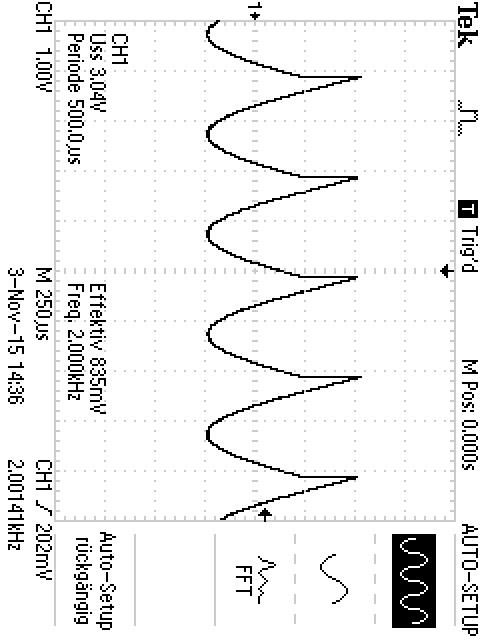
\includegraphics[angle=90,height=2.6cm]{graphics/ALL0034/F0034TEK.jpg}
\label{fig:phi180o}
\end{subfigure}
\begin{subfigure}{0.48\textwidth}
\centering
\caption*{mit Rauschen:}
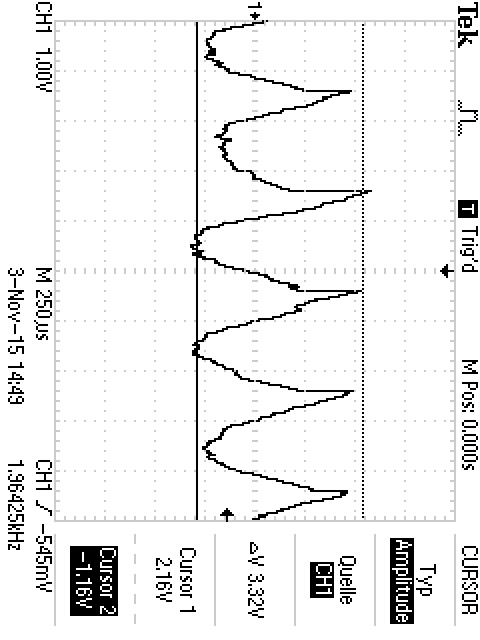
\includegraphics[angle=90,height=2.6cm]{graphics/ALL0042/F0042TEK.jpg}
\label{fig:phi180m}
\end{subfigure}
\end{figure}
\addtocounter{figure}{-1}
\begin{figure}
\caption{$U_{out} (\phi = 210°$)}
\begin{subfigure}{0.48\textwidth}
\centering
\caption*{ohne Rauschen:}
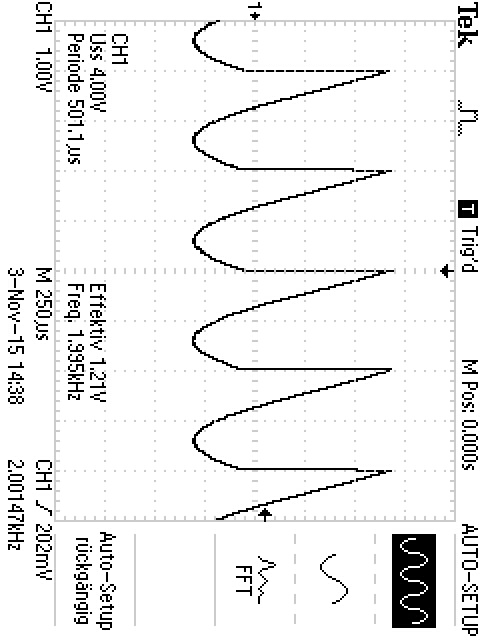
\includegraphics[angle=90,height=2.6cm]{graphics/ALL0036/F0036TEK.jpg}
\label{fig:phi210o}
\end{subfigure}
\begin{subfigure}{0.48\textwidth}
\centering
\caption*{mit Rauschen:}
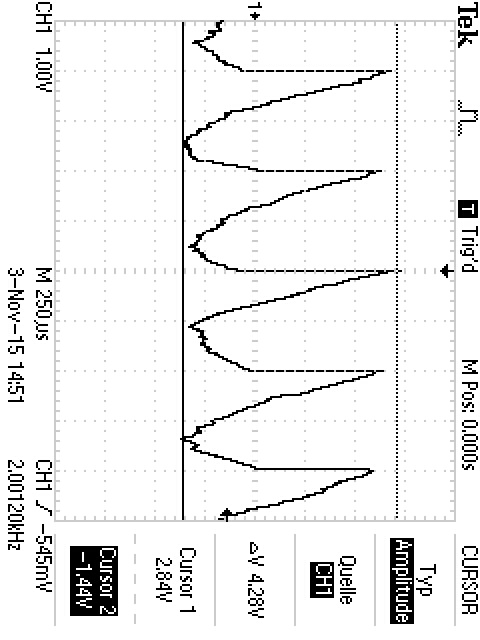
\includegraphics[angle=90,height=2.6cm]{graphics/ALL0044/F0044TEK.jpg}
\label{fig:phi210m}
\end{subfigure}
\end{figure}
\addtocounter{figure}{-1}
\begin{figure}
\caption{$U_{out} (\phi = 270°$)}
\begin{subfigure}{0.48\textwidth}
\centering
\caption*{ohne Rauschen:}
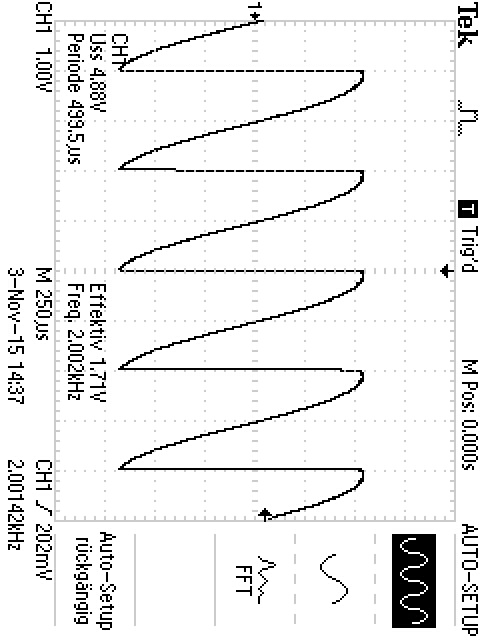
\includegraphics[angle=90,height=2.6cm]{graphics/ALL0035/F0035TEK.jpg}
\label{fig:phi270o}
\end{subfigure}
\begin{subfigure}{0.48\textwidth}
\centering
\caption*{mit Rauschen:}
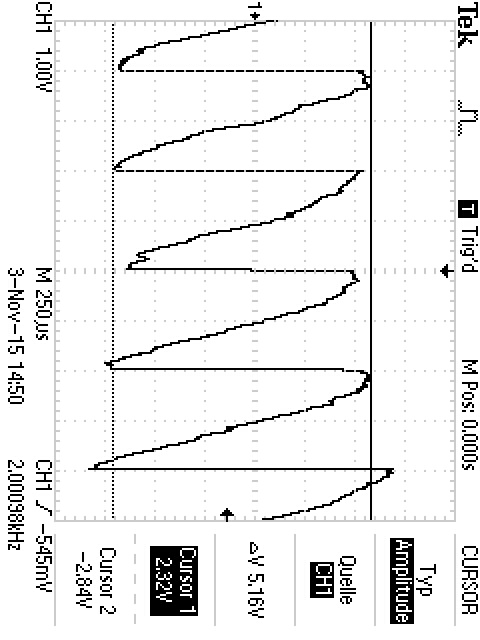
\includegraphics[angle=90,height=2.6cm]{graphics/ALL0043/F0043TEK.jpg}
\label{fig:phi270m}
\end{subfigure}
\end{figure}
\addtocounter{figure}{-1}
\begin{figure}
\caption{$U_{out} (\phi = 340°$) }
\begin{subfigure}{0.48\textwidth}
\centering
\caption*{ohne Rauschen:}
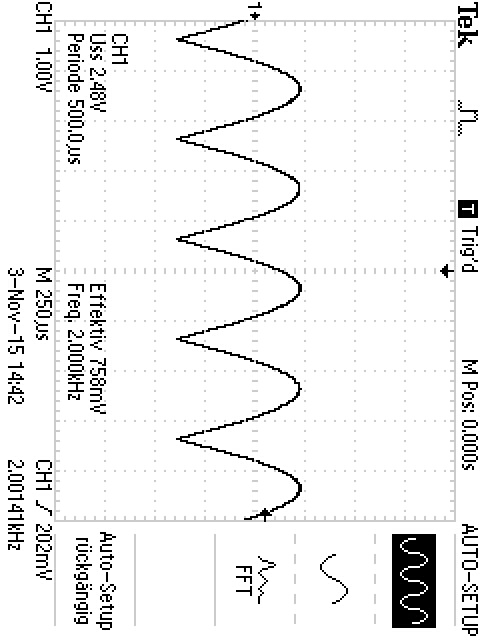
\includegraphics[angle=90,height=2.6cm]{graphics/ALL0038/F0038TEK.jpg}
\label{fig:phi340o}
\end{subfigure}
\begin{subfigure}{0.48\textwidth}
\centering
\caption*{mit Rauschen:}
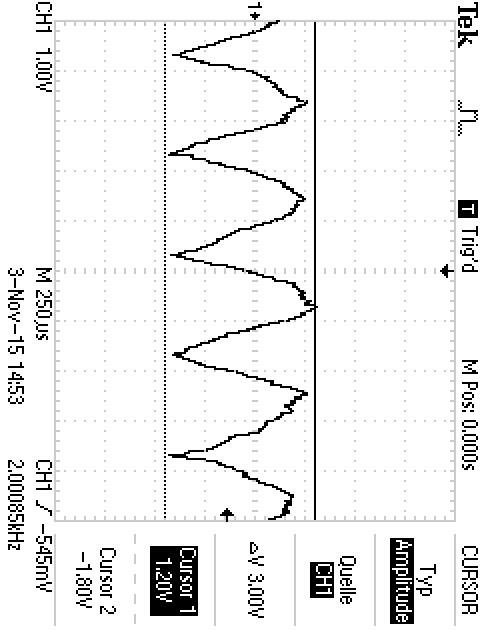
\includegraphics[angle=90,height=2.6cm]{graphics/ALL0046/F0046TEK.jpg}
\label{fig:phi340m}
\end{subfigure}
\label{fig:U_out}
\end{figure}
\addtocounter{figure}{-1}

\newpage

\captionsetup{labelformat=default}

\subsection{Auswertung: LED und Photodiode}



In \ref{fig:plot4} ist das am Tiefpaß integrierte Signal in Abhängigkeit von
dem Abstand $r$ zwischen LED und Photodiode dargestellt, wobei das Umgebungslicht
die Messung als Rauschen verfälscht. Das erwartete Ergebnis
ist, dass die Spannung mit steigendem Abstand abnimmt. Interessanterweise
sind die 1,86m der Versuchsapparatur allerding nicht genug um die Intensität
des Lichts der LED soweit abzuschwächen, dass die Photodiode kein Signal
mehr detektieren könnte. Bei diesem maximalen Abstand ist am Tiefpaß noch ein
Wert von 0,5 (mit Gain = 1000) abzulesen. Wenn der Weg zwischen LED und
Diode unterbrochen wird (z.B. indem eine Hand vor die LED gehalten wird),
sodass die Diode kein Licht der LED mehr empfangen kann, ergibt sich am
Tiefpaß ein Wert von 0,2 (mit Gain = 1000). Das zeigt, dass die Diode auch
bei $r$=1,86m noch Licht der LED empfängt, dass mit dem Lock-In-Verstärker
ausgewertet werden kann.
\begin{figure}
  \centering
  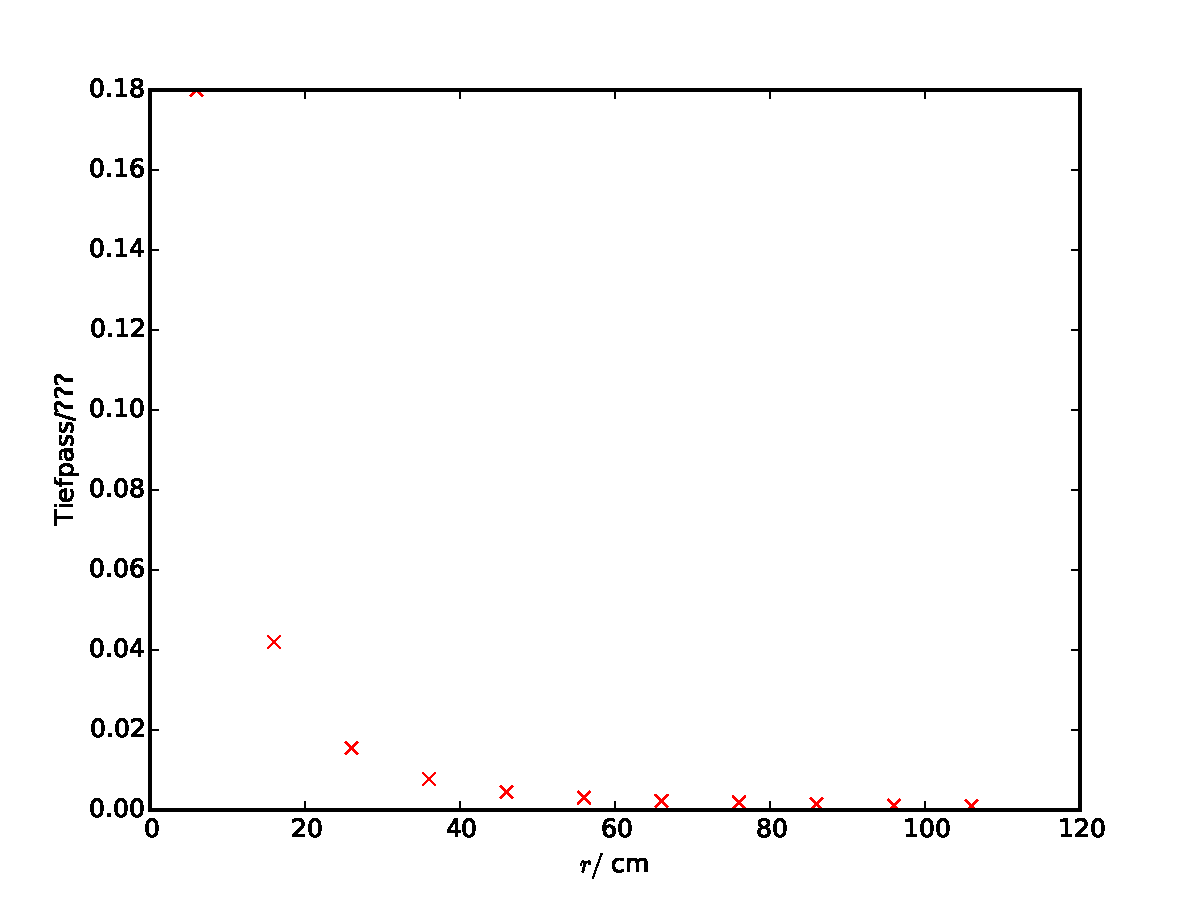
\includegraphics[width=0.8\textwidth, height=0.5\textwidth]{plot4.pdf}
  \caption{Integriertes Signal}
  \label{fig:plot4}
\end{figure}
